\PassOptionsToPackage{dvipsnames,svgnames,x11names}{xcolor}
\documentclass[portrait,a0paper,fontscale=0.312]{baposter}

% For graphs
\usepackage{graphicx}

\usepackage{array}
\usepackage{booktabs}
\usepackage{eso-pic}
\usepackage{layout}
\usepackage{fancybox}


\usepackage{calc}
\usepackage{amsmath}
\usepackage{amssymb}
\usepackage{relsize}
\usepackage{multirow}
\usepackage{rotating}
\usepackage{bm}
\usepackage{url}
\usepackage{xfrac}
\usepackage{natbib}
\usepackage{mathtools}
\usepackage{cancel}
\usepackage{paralist}
\usepackage{subfigure}

% \usepackage[centering,includeheadfoot,margin=2cm]{geometry}

\usepackage{multicol}

% \usepackage[linesnumbered,ruled,vlined,noend]{algorithm2e}
% % \usepackage{algorithmicx}
% % \usepackage{algpseudocode}
% \newlength\figureheight
% \newlength\figurewidth
% \setlength{\algomargin}{2em}
% \SetKwComment{Comment}{$\blacktriangleright$\ }{}
% 
% \providecommand{\SetAlgoLined}{\SetLine}
% \providecommand{\DontPrintSemicolon}{\dontprintsemicolon}

\newcommand{\figurewidth}{7cm}
\newcommand{\figureheight}{3cm}

%\usepackage{times}
%\usepackage{helvet}
%\usepackage{bookman}
\usepackage{palatino}

\newcommand{\captionfont}{\footnotesize}

\usetikzlibrary{calc}

% \newcommand{\SET}[1]  {\ensuremath{\mathcal{#1}}}
% \newcommand{\MAT}[1]  {\ensuremath{\boldsymbol{#1}}}
% \newcommand{\VEC}[1]  {\ensuremath{\boldsymbol{#1}}}
% \newcommand{\Video}{\SET{V}}
% \newcommand{\video}{\VEC{f}}
% \newcommand{\track}{x}
% \newcommand{\Track}{\SET T}
% \newcommand{\LMs}{\SET L}
% \newcommand{\lm}{l}
% \newcommand{\PosE}{\SET P}
% \newcommand{\posE}{\VEC p}
% \newcommand{\negE}{\VEC n}
% \newcommand{\NegE}{\SET N}
% \newcommand{\Occluded}{\SET O}
% \newcommand{\occluded}{o}

\renewcommand{\sfdefault}{lmss}
\sffamily


\newcommand{\listhead}[1] {\textsc{\underline{#1}}}

\definecolor{rouge1}{RGB}{226,0,38}  % red P
\definecolor{orange1}{RGB}{243,154,38}  % orange P
\definecolor{jaune}{RGB}{254,205,27}  % jaune P
\definecolor{blanc}{RGB}{255,255,255} % blanc P

\definecolor{rouge2}{RGB}{230,68,57}  % red S
\definecolor{orange2}{RGB}{236,117,40}  % orange S
\definecolor{taupe}{RGB}{134,113,127} % taupe S
\definecolor{gris}{RGB}{91,94,111} % gris S
\definecolor{bleu1}{RGB}{38,109,131} % bleu S
\definecolor{bleu2}{RGB}{28,50,114} % bleu S
\definecolor{vert1}{RGB}{133,146,66} % vert S
\definecolor{vert3}{RGB}{20,200,66} % vert S
\definecolor{vert2}{RGB}{157,193,7} % vert S
\definecolor{darkyellow}{RGB}{233,165,0}  % orange S
\definecolor{lightgray}{rgb}{0.9,0.9,0.9}
\definecolor{darkgray}{rgb}{0.6,0.6,0.6}

\definecolor{blue900}{HTML}{0D47A1}
\definecolor{blue800}{HTML}{1565C0}

\newcommand{\rcol}[1]{\textcolor{red}{\textit{#1}}}
\newcommand{\gcol}[1]{\textcolor{vert3}{\textit{#1}}}
\newcommand{\bcol}[1]{\textcolor{blue}{\textit{#1}}}
\newcommand{\ycol}[1]{\textcolor{darkyellow}{\textit{#1}}}

\newcommand{\rcolb}[1]{\textcolor{red}{\textit{\textbf{#1}}}}
\newcommand{\gcolb}[1]{\textcolor{vert3}{\textit{\textbf{#1}}}}
\newcommand{\bcolb}[1]{\textcolor{blue}{\textit{\textbf{#1}}}}
\newcommand{\ycolb}[1]{\textcolor{darkyellow}{\textit{\textbf{#1}}}}

\newcommand{\otoprule}{\midrule[\heavyrulewidth]}
\newcommand{\dbacks}[1]{\textbf{\textcolor{red!80!black}{{#1}}}}


\usepackage{tikz,pgfplots}
\pgfplotsset{compat=newest}
\tikzstyle{every picture}+=[remember picture]
\tikzstyle{na} = [baseline=-.5ex]
\everymath{\displaystyle}
\usetikzlibrary{arrows,shapes}
\usetikzlibrary{positioning}

\usepackage{wasysym}

%%%%%%%%%%%%%% COMMANDS
\newcommand{\alg}{RQ-Learning\xspace}

\newcommand{\Rmodel}{\mathcal{R}}
\newcommand{\Pmodel}{\mathcal{P}}
\newcommand{\Rparams}[1][]{\boldsymbol{\omega}^{#1}}
\newcommand{\Rpspace}{\Omega}
\newcommand{\Rbasis}[1][]{\boldsymbol{\phi}\left({#1}\right)}
\newcommand{\Rmodelp}[1][\Rparams]{\mathcal{R}^{#1}}
\newcommand{\Rspace}[1][\dobj-1]{\Delta^{#1}}
\newcommand{\Simplex}[1][\dobj-1]{\mathbb{D}^{#1}}
\newcommand{\Rparamsdom}{\Theta^{*}}

\newcommand{\dsetexp}{\mathcal{D}}
\newcommand{\numdsetexp}{N}

\newcommand{\fe}[2][]{\boldsymbol{\mu}_{#2}\left(#1\right)}  %feature expectation
\newcommand{\feapx}{\widehat{\boldsymbol{\mu}}}                %approximate fe
\newcommand{\jval}[2][]{J_{#2}\left({#1}\right)}
\newcommand{\djval}[2][]{\Delta J_{#2}\left({#1}\right)}
\newcommand{\poly}{\mathcal{P}}
\newcommand{\radius}{r}
\newcommand{\acval}{\rho}
\newcommand{\targetset}{\mathbb{X}^{\epsilon}}

\newcommand{\dpolycut}{m}

\newcommand{\JvalMO}[2][\pi]{\boldsymbol{J}_{#2}\left(#1\right)}
%%%%%%%%%%%%%%%%%%%%%%%



%% math commands
\newcommand{\transpose}[1]{{#1}^\texttt{T}}
\DeclareMathOperator*{\argmax}{arg\,max}
\DeclareMathOperator*{\argmin}{arg\,min}
\DeclareMathOperator*{\EV}{\mathbb{E}}
\DeclareMathOperator*{\var}{\textbf{\texttt{Var}}}
\DeclareMathOperator*{\gradp}{\nabla_{\ppvect}}
\DeclareMathOperator*{\gradhp}{\nabla_{\hpvect}}

\newcommand{\norm}[2][\infty]{\left\|#2\right\|_{#1}}

\newcommand{\realspace}{\mathbb R}		% realspace

\newcommand{\statespace}{\mathcal X}		% state space
\newcommand{\actionspace}{\mathcal U}		% action space
\newcommand{\pmodel}{\mathcal P}		% transition function
\newcommand{\rmodel}{\mathcal R}		% reward function
\newcommand{\initD}{D}				% initial distribution

%% Vector and Matrix
\newcommand{\rvect}{\mathbf{R}}			% reward vector
\newcommand{\vvect}{\mathbf{V}}			% value function vector
\newcommand{\jvect}{\mathbf{J}}			% score vector
\newcommand{\gammavect}{\boldsymbol{\gamma}}	% gamma vector
\newcommand{\pmtx}{\mathbf{P}}			% transition matrix


\newcommand{\ppspace}{\Theta}
\newcommand{\pp}{\theta} 			% policy params
\newcommand{\ppvect}{\boldsymbol{\pp}}		% policy params vector (bold)
\newcommand{\vecop}{\text{vec }}
\newcommand{\sap}{\boldsymbol{z}}

\newcommand{\hpvect}{\boldsymbol \rho}
\newcommand{\hyperdist}{}

\newcommand{\Jvalapx}[1][\ppvect]{\widehat{J}\left({#1}\right)}
\newcommand{\Jval}[1][\ppvect]{J\left({#1}\right)}
\newcommand{\Jvalp}[2][\ppvect]{J_{#2}\left({#1}\right)}
\newcommand{\Mval}[1][\ppvect]{M\left({#1}\right)}
\newcommand{\Jvalvect}[1][\ppvect]{\jvect\left({#1}\right)}
\newcommand{\offJval}[1][\ppvect]{\mathcal{J}\left({#1}\right)}

\newcommand{\dstate}{n}
\newcommand{\daction}{m}
\newcommand{\dobj}{q}
\newcommand{\dpolicy}{d}

\newcommand{\numtraj}{N}

\newcommand{\horiz}{T}
\newcommand{\traj}{\tau}
\newcommand{\trajset}{\mathcal{T}}
\newcommand{\trajspace}{\mathbb{T}}
\newcommand{\trajlength}{T}
\newcommand{\trajR}{R}
\newcommand{\pdfunc}[1]{p\left(#1\right)}

\newcommand{\currstep}{t}	% index for current time step in GPOMDP derivations
\newcommand{\indxlogpi}{i}	% index for \sum \nabla log policy
\newcommand{\indxr}{j}		% index for \sum reward
\newcommand{\indxis}{w}		% index  for \prod importance sampling
\newcommand{\indxint}{k}	% index for \prod \int
\newcommand{\indxcomp}{k}	% index for \theta or gradient components
\newcommand{\indxcompr}{h}	% index for reward or gradient components

\newcommand{\Hessian}{\mathcal{H}}
\newcommand{\HJ}[1][\ppvect]{\Hessian_{\ppvect}\jvect({#1})}
\newcommand{\HJhat}[1][\ppvect]{\widehat{\Hessian}_{\ppvect}\jvect({#1})}
\newcommand{\HJREF}[1][\ppvect]{\widehat{\Hessian}_{\ppvect}^{RF}\jvect({#1})}
\newcommand{\HJGP}[1][\ppvect]{\widehat{\Hessian}_{\ppvect}^{GP}\jvect({#1})}
\newcommand{\glp}[1][]{\nabla_{\ppvect} \log \pi_{\ppvect}(a_{#1}|s_{#1})}
\newcommand{\hlp}[1][]{H_{\ppvect} \log \pi_{\ppvect}(a_{#1}|s_{#1})}

\newcommand{\EVV}[2][\ppvect \in \ppspace]{\EV_{#1}\left[{#2}\right]}
\newcommand{\EVVC}[3]{\EV_{\substack{#1}}\left[{#2}\middle|{#3}\right]}

\newcommand{\cMtx}[1][]{\mathcal{C}\left(#1\right)}
\newcommand{\basegrad}{b_{\nabla}}
\newcommand{\baseline}{b_\indxcomp}
\newcommand{\stepbaseline}{b^{(\currstep)}_\indxcomp}
\newcommand{\baseF}{F^{(\traj)}}
\newcommand{\baseG}{G_\indxcomp^{(\traj)}}
\newcommand{\stepbaseF}{F^{(\currstep)}}
\newcommand{\stepbaseG}{G_\indxcomp^{(\currstep)}}
\newcommand{\varr}[1][]{\textbf{\texttt{Var}}\left( {#1}\right)}

\newcommand{\pol}{\pi}
\newcommand{\polb}{\pi^{\mathcal{B}}}
\newcommand{\polt}{\pi^{\mathcal{T}}}

\newcommand{\qf}[1][^\pol]{Q#1}
\newcommand{\qffun}[2]{Q#1\left(#2\right)}		% value function with parenthesis

\newcommand{\mow}{\boldsymbol{\alpha}}
% \newcommand{\mow}{\Rparams}

\newcommand{\normv}{x}
\newcommand{\normpow}{y}
\newcommand{\ncost}[1][_{\normv}^{\normpow}]{\mathcal{C}{#1}}

\newcommand{\mdp}{\mathcal{M}}

\newcommand{\texsub}[1]{\textsc{\tiny #1}}


\usepackage{xspace}
\DeclareRobustCommand{\eg}{e.g.,\@\xspace}
\DeclareRobustCommand{\ie}{i.e.,\@\xspace}
\DeclareRobustCommand{\wrt}{w.r.t.\@\xspace}

%%
\newtheorem{Property}{Property}
\newtheorem{theorem}{Theorem}

% Q decomposition commands
\newcommand{\Rtilde}{\widetilde{R}}
\newcommand{\Qtilde}{\widetilde{Q}}

%%%%%%%%%%%%%%% COMMANDS

\newcommand{\Rmodel}{\mathcal{R}}
\newcommand{\Pmodel}{\mathcal{P}}
\newcommand{\Rparams}[1][]{\boldsymbol{\omega}^{#1}}
\newcommand{\Rbasis}[1][]{\boldsymbol{\phi}\left({#1}\right)}
\newcommand{\Rmodelp}[1][\Rparams]{\mathcal{R}^{#1}}
\newcommand{\Rspace}[1][\dobj-1]{\Delta^{#1}}
\newcommand{\Simplex}[1][\dobj-1]{\mathbb{D}^{#1}}
\newcommand{\Rparamsdom}{\Theta^{*}}

\newcommand{\dsetexp}{\mathcal{D}}
\newcommand{\numdsetexp}{N}

\newcommand{\fe}[2][]{\boldsymbol{\mu}_{#2}\left(#1\right)}  %feature expectation
\newcommand{\feapx}{\widehat{\boldsymbol{\mu}}}                %approximate fe
\newcommand{\jval}[2][]{J_{#2}\left({#1}\right)}
\newcommand{\djval}[2][]{\Delta J_{#2}\left({#1}\right)}
\newcommand{\poly}{\mathcal{P}}
\newcommand{\radius}{r}
\newcommand{\acval}{\rho}
\newcommand{\targetset}{\mathbb{X}^{\epsilon}}

\newcommand{\dpolycut}{m}

\newcommand{\JvalMO}[2][\pi]{\boldsymbol{J}_{#2}\left(#1\right)}
%%%%%%%%%%%%%%%%%%%%%%%
\usepackage{tcolorbox}


%%%%%%%%%%%%%%%%%%%%%%%%%%%%%%%%%%%%%%%%%%%%%%%%%%%%%%%%%%%%%%%%%%%%%%%%%%%%%%%%
%%%% Some math symbols used in the text
%%%%%%%%%%%%%%%%%%%%%%%%%%%%%%%%%%%%%%%%%%%%%%%%%%%%%%%%%%%%%%%%%%%%%%%%%%%%%%%%

%%%%%%%%%%%%%%%%%%%%%%%%%%%%%%%%%%%%%%%%%%%%%%%%%%%%%%%%%%%%%%%%%%%%%%%%%%%%%%%%
% Multicol Settings
%%%%%%%%%%%%%%%%%%%%%%%%%%%%%%%%%%%%%%%%%%%%%%%%%%%%%%%%%%%%%%%%%%%%%%%%%%%%%%%%
\setlength{\columnsep}{1.5em}
\setlength{\columnseprule}{0mm}

%%%%%%%%%%%%%%%%%%%%%%%%%%%%%%%%%%%%%%%%%%%%%%%%%%%%%%%%%%%%%%%%%%%%%%%%%%%%%%%%
% Save space in lists. Use this after the opening of the list
%%%%%%%%%%%%%%%%%%%%%%%%%%%%%%%%%%%%%%%%%%%%%%%%%%%%%%%%%%%%%%%%%%%%%%%%%%%%%%%%
\newcommand{\compresslist}{%
\setlength{\itemsep}{1pt}%
\setlength{\parskip}{0pt}%
\setlength{\parsep}{0pt}%
}

%%%%%%%%%%%%%%%%%%%%%%%%%%%%%%%%%%%%%%%%%%%%%%%%%%%%%%%%%%%%%%%%%%%%%%%%%%%%%%
%%% Begin of Document
%%%%%%%%%%%%%%%%%%%%%%%%%%%%%%%%%%%%%%%%%%%%%%%%%%%%%%%%%%%%%%%%%%%%%%%%%%%%%%

\begin{document}

%%%%%%%%%%%%%%%%%%%%%%%%%%%%%%%%%%%%%%%%%%%%%%%%%%%%%%%%%%%%%%%%%%%%%%%%%%%%%%
%%% Here starts the poster
%%%---------------------------------------------------------------------------
%%% Format it to your taste with the options
%%%%%%%%%%%%%%%%%%%%%%%%%%%%%%%%%%%%%%%%%%%%%%%%%%%%%%%%%%%%%%%%%%%%%%%%%%%%%%
% Define some colors

%\definecolor{lightblue}{cmyk}{0.83,0.24,0,0.12}
\definecolor{lightblue}{rgb}{0.145,0.6666,1}

% % Draw a video
% \newlength{\FSZ}
% \newcommand{\drawvideo}[3]{% [0 0.25 0.5 0.75 1 1.25 1.5]
%    \noindent\pgfmathsetlength{\FSZ}{\linewidth/#2}
%    \begin{tikzpicture}[outer sep=0pt,inner sep=0pt,x=\FSZ,y=\FSZ]
%    \draw[color=lightblue!50!black] (0,0) node[outer sep=0pt,inner sep=0pt,text width=\linewidth,minimum height=0] (video) {\noindent#3};
%    \path [fill=lightblue!50!black,line width=0pt] 
%      (video.north west) rectangle ([yshift=\FSZ] video.north east) 
%     \foreach \x in {1,2,...,#2} {
%       {[rounded corners=0.6] ($(video.north west)+(-0.7,0.8)+(\x,0)$) rectangle +(0.4,-0.6)}
%     }
% ;
%    \path [fill=lightblue!50!black,line width=0pt] 
%      ([yshift=-1\FSZ] video.south west) rectangle (video.south east) 
%     \foreach \x in {1,2,...,#2} {
%       {[rounded corners=0.6] ($(video.south west)+(-0.7,-0.2)+(\x,0)$) rectangle +(0.4,-0.6)}
%     }
% ;
%    \foreach \x in {1,...,#1} {
%      \draw[color=lightblue!50!black] ([xshift=\x\linewidth/#1] video.north west) -- ([xshift=\x\linewidth/#1] video.south west);
%    }
%    \foreach \x in {0,#1} {
%      \draw[color=lightblue!50!black] ([xshift=\x\linewidth/#1,yshift=1\FSZ] video.north west) -- ([xshift=\x\linewidth/#1,yshift=-1\FSZ] video.south west);
%    }
%    \end{tikzpicture}
% }
% 
% \hyphenation{resolution occlusions}
% %%
\begin{poster}%
  % Poster Options
  {
  % Show grid to help with alignment
  columns=6,
  grid=false,
  % Column spacing
  colspacing=1em,
  % Color style
  bgColorOne=white,
  bgColorTwo=white,
  borderColor=blue900,
  headerColorOne=blue800,
  headerColorTwo=blue800,
  headerFontColor=white,
  boxColorOne=white,
  boxColorTwo=lightblue,
  % Format of textbox
  textborder=roundedleft,
  % Format of text header
  eyecatcher=true,
  headerborder=closed,
  headerheight=0.1\textheight,
%  textfont=\sc, An example of changing the text font
  headershape=roundedright,
  headershade=shadelr,
  headerfont=\Large\bf\textsc, %Sans Serif
  textfont={\setlength{\parindent}{1.5em}},
  boxshade=plain,
%  background=shade-tb,
  background=plain,
  linewidth=2pt
  }
  % Eye Catcher
  {
\includegraphics[height=9em]{./pics/airlab_logo_reflect.png}} 
%   {\hspace{3.5cm}}
  % Title
  {\bf\textsc{Exploiting Structure and Uncertainty of Bellman Updates in Markov Decision Processes}\vspace{0.1em}}
  % Authors
  {\textsc{D. Tateo, C. D'Eramo, A. Nuara, M. Restelli, A. Bonarini}\\ {\normalsize \texttt{\{davide.tateo, carlo.deramo, alessandro.nuara, marcello.restelli, andrea.bonarini\}@polimi.it}}}
  % University logo
  {% The makebox allows the title to flow into the logo, this is a hack because of the L shaped logo.
    %
\includegraphics[height=9.0em]{./pics/PoliMI.pdf}%\hspace{.5cm}
    
\includegraphics[height=9.0em]{./pics/polilogo/logoPoliBlue_poster.png}
  }

%%%%%%%%%%%%%%%%%%%%%%%%%%%%%%%%%%%%%%%%%%%%%%%%%%%%%%%%%%%%%%%%%%%%%%%%%%%%%%
%%% Now define the boxes that make up the poster
%%%---------------------------------------------------------------------------
%%% Each box has a name and can be placed absolutely or relatively.
%%% The only inconvenience is that you can only specify a relative position 
%%% towards an already declared box. So if you have a box attached to the 
%%% bottom, one to the top and a third one which should be in between, you 
%%% have to specify the top and bottom boxes before you specify the middle 
%%% box.
%%%%%%%%%%%%%%%%%%%%%%%%%%%%%%%%%%%%%%%%%%%%%%%%%%%%%%%%%%%%%%%%%%%%%%%%%%%%%%
    %
    % A coloured circle useful as a bullet with an adjustably strong filling
    \newcommand{\colouredcircle}{%
      \tikz{\useasboundingbox (-0.2em,-0.32em) rectangle(0.2em,0.32em); \draw[draw=black,fill=lightblue,line width=0.03em] (0,0) circle(0.18em);}}

\newcommand{\HL}[1]{\textcolor{blue}{\textbf{#1}}}

%%%%%%%%%%%%%%%%%%%%%%%%%%%%%%%%%%%%%%%%%%%%%%%%%%%%%%%%%%%%%%%%%%%%%%%%%%%%%%
  \headerbox{Contributions}{name=contributions,column=3,row=0, span=3}{
%%%%%%%%%%%%%%%%%%%%%%%%%%%%%%%%%%%%%%%%%%%%%%%%%%%%%%%%%%%%%%%%%%%%%%%%%%%%%%
% \vspace{-0.2cm}
\begin{enumerate}\compresslist
\item Split the estimate in two components:
  \begin{itemize}
   \item The expected reward $\Rtilde(x,u)$
   \item The expected next state value function $\Qtilde(x,u)$
  \end{itemize}
\item Use different learning rates for the two components
\item We provide empirical results showing the effectiveness of our approach

\end{enumerate}
  }


%%%%%%%%%%%%%%%%%%%%%%%%%%%%%%%%%%%%%%%%%%%%%%%%%%%%%%%%%%%%%%%%%%%%%%%%%%%%%%
  \headerbox{Problem}{name=problem,column=0,row=0,span=3, bottomaligned=contributions}{
%%%%%%%%%%%%%%%%%%%%%%%%%%%%%%%%%%%%%%%%%%%%%%%%%%%%%%%%%%%%%%%%%%%%%%%%%%%%%%
\begin{itemize}\compresslist
 \item Learning is difficult in highly stochastic environments
 \item Uncertainty in action-value function estimates propagates
 \item Some algorithms face this problem focusing on the bias of the estimate
\end{itemize}
  }
  
% %%%%%%%%%%%%%%%%%%%%%%%%%%%%%%%%%%%%%%%%%%%%%%%%%%%%%%%%%%%%%%%%%%%%%%%%%%%%%%
%   \headerbox{Settings}{name=settings,column=4,row=0,span=2,bottomaligned=contributions}{
% %%%%%%%%%%%%%%%%%%%%%%%%%%%%%%%%%%%%%%%%%%%%%%%%%%%%%%%%%%%%%%%%%%%%%%%%%%%%%%
% 
% \renewcommand{\CancelColor}{\color{red}}
% \noindent \textbf{MDP without reward:} $\mdp = \langle\statespace,\actionspace, \pmodel, \xcancel{\rmodel}, \gamma \rangle$
% 
% }

%%%%%%%%%%%%%%%%%%%%%%%%%%%%%%%%%%%%%%%%%%%%%%%%%%%%%%%%%%%%%%%%%%%%%%%%%%%%%%
  \headerbox{RQ-Learning Algorithm}{name=rq,column=0,span=6,row=3,below=contributions}{
%%%%%%%%%%%%%%%%%%%%%%%%%%%%%%%%%%%%%%%%%%%%%%%%%%%%%%%%%%%%%%%%%%%%%%%%%%%%%%
%\hspace{.5cm}
\hfill
\begin{minipage}[t]{.47\textwidth}
  \listhead{Idea}\\
  Split the action-value function in two components:
  \begin{itemize}\compresslist
    \renewcommand{\CancelColor}{\color{red}}
    \item $\Rtilde(x,u)=\underset{\strut\mathclap{x'\sim \Pmodel(x'|x,u)}}{\mathbb{E}}\left[ r(x,u,x')\right]$
    \item $\Qtilde(x,u)=\underset{\strut\mathclap{x'\sim \Pmodel(x'|x,u)}}{\mathbb{E}}\left[\max_{u'} Q^*(x',u')\right]$
    \item $Q^*(x,u)=\Rtilde(x,u)+\gamma\Qtilde(x,u)$
  \end{itemize}
  Compute the update as follows:
  \begin{itemize}
    \item $\Rtilde_{t+1}(x,u) \leftarrow\Rtilde_t(x,u)+\alpha_t(R(x,u,x')-\Rtilde_t(x,u))$
    \item $\Qtilde_{t+1}(x,u) \leftarrow\Qtilde_t(x,u)+\beta_t(\max_{u'}Q_t(x',u')-\Qtilde_t(x,u))$
  \end{itemize}
  
  Different effects on the choiche of $\alpha$ and $\beta$:
  \begin{description}
    \item[Q-Learning] $\alpha_t=\beta_t$
    \item[$\text{RQ}_\delta$-Learning] $\beta_t=\alpha_t\delta_t$
    \item[RQ-Learning] $\beta_t\neq\alpha_t$
  \end{description}
\end{minipage}% <-- Don't forget this one
%
\hfill
%
\begin{minipage}[t]{.47\textwidth}
  \listhead{Learning rate on the variance of the estimation}\\
  Exploit the variance of estimation to set the learning rate:
    \begin{enumerate}
   \item Estimate the variance of the estimator $\Qtilde$, using the sample variance of the target:\\
   $\mathrm{Var}\left[\Qtilde\right]=S_t^2\omega_t$ \\
   $\omega_{t+1}=(1-\beta_t)^2\omega_t+\beta_t^2$ \\
   
   \item Compute the learning rate
      \begin{itemize}
	\item Select a $\beta$ that decreases when the estimate precision increases:\\
	$\beta_t=\dfrac{\sigma_e^2(t)}{\sigma_e^2(t)+\eta}$
	\item Or, select a $\delta$ that increases when the estimate precision increases: \\
	$\delta_t=e^{\frac{\sigma_e^2}{\eta}\log\frac{1}{2}}$
      \end{itemize}
  \end{enumerate}

\end{minipage}
\hfill
}

%%%%%%%%%%%%%%%%%%%%%%%%%%%%%%%%%%%%%%%%%%%%%%%%%%%%%%%%%%%%%%%%%%%%%%%%%%%%%%
\headerbox{Empirical Results}{name=emp,column=0,row=3,span=6,below=rq}{
% \headerbox{Finite Sample Analysis}{name=settings,column=2,row=0}{
%%%%%%%%%%%%%%%%%%%%%%%%%%%%%%%%%%%%%%%%%%%%%%%%%%%%%%%%%%%%%%%%%%%%%%%%%%%%%%

\listhead{Noisy Gridworld}\\
\begin{minipage}{0.5\textwidth}
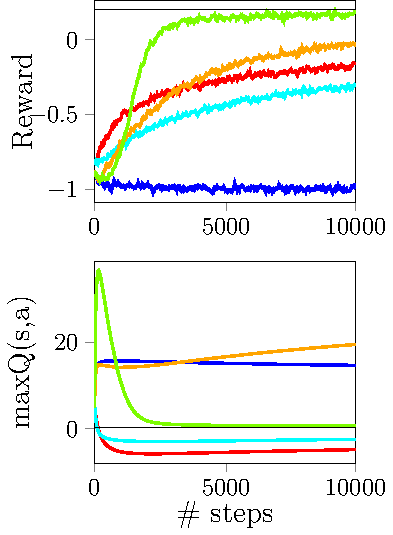
\includegraphics[scale=0.55]{./imgs/gridHasselt/allAlgs1.pdf}
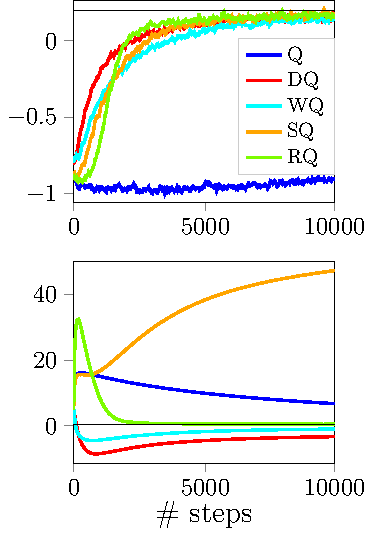
\includegraphics[scale=0.55]{./imgs/gridHasselt/allAlgs08.pdf}
\end{minipage}%
%
\hfill
%
\begin{minipage}{0.5\textwidth}
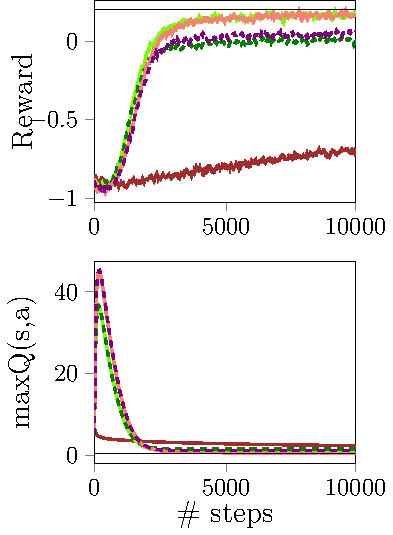
\includegraphics[scale=0.55]{./imgs/gridHasselt/QDecs1.pdf}
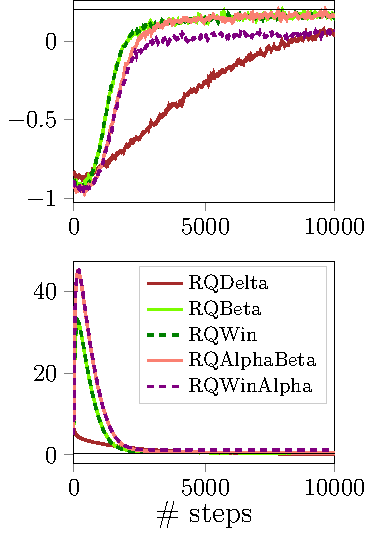
\includegraphics[scale=0.55]{./imgs/gridHasselt/QDecs08.pdf}
\end{minipage}

\listhead{Double chain}\\
\begin{minipage}{0.5\textwidth}
  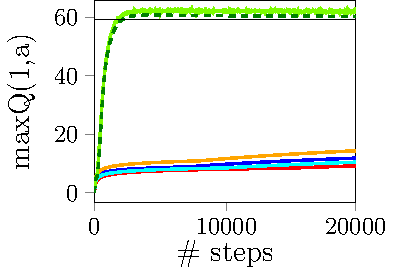
\includegraphics[scale=0.55]{./imgs/doubleChain/v1-1.pdf}
  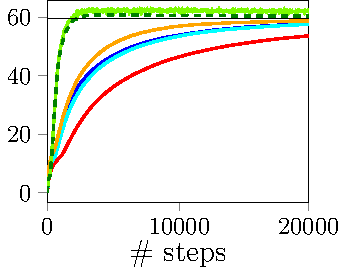
\includegraphics[scale=0.55]{./imgs/doubleChain/v1-51.pdf}\\
  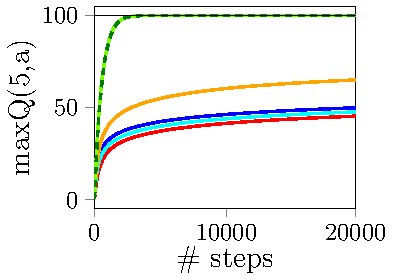
\includegraphics[scale=0.55]{./imgs/doubleChain/v5-1.pdf}
  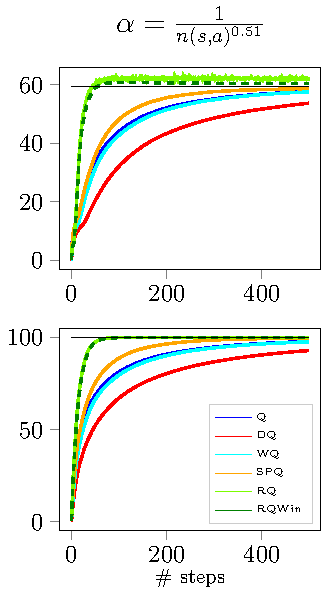
\includegraphics[scale=0.55]{./imgs/doubleChain/v5-51.pdf}
\end{minipage} %
%
\hfill
%
\begin{minipage}{0.5\textwidth}
  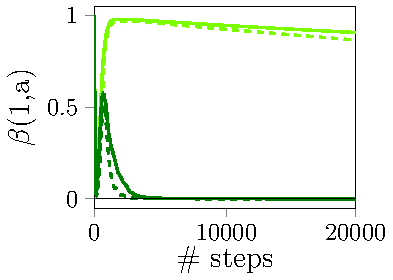
\includegraphics[scale=0.55]{./imgs/doubleChain/lrs1-1.pdf}
  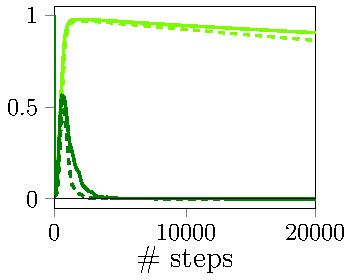
\includegraphics[scale=0.55]{./imgs/doubleChain/lrs1-51.pdf}\\
  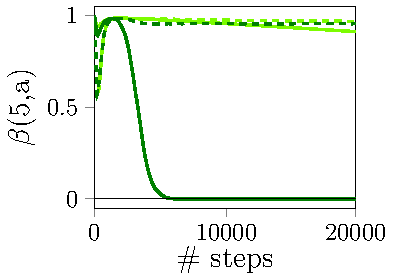
\includegraphics[scale=0.55]{./imgs/doubleChain/lrs5-1.pdf}
  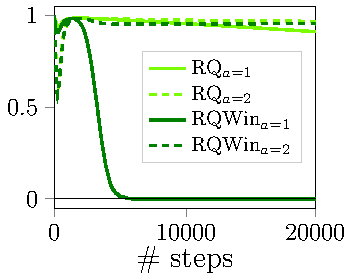
\includegraphics[scale=0.55]{./imgs/doubleChain/lrs5-51.pdf}
\end{minipage}

\listhead{Gridworld with Holes}\\
{\centering
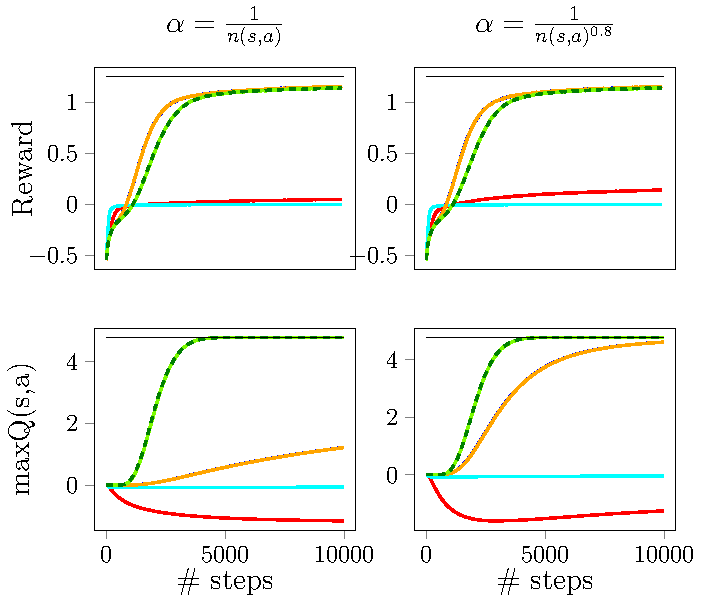
\includegraphics[scale=0.55]{./imgs/gridHole/grid_hole.pdf}
}
}
% 
% %%%%%%%%%%%%%%%%%%%%%%%%%%%%%%%%%%%%%%%%%%%%%%%%%%%%%%%%%%%%%%%%%%%%%%%%%%%%%%
% \headerbox{Results}{name=results,column=2,row=3,below=fsa,bottomaligned=btt}{
% % \headerbox{Results}{name=results,column=2,row=3,below=fsa,above=bottom}{
% %%%%%%%%%%%%%%%%%%%%%%%%%%%%%%%%%%%%%%%%%%%%%%%%%%%%%%%%%%%%%%%%%%%%%%%%%%%%%%
% }

% %%%%%%%%%%%%%%%%%%%%%%%%%%%%%%%%%%%%%%%%%%%%%%%%%%%%%%%%%%%%%%%%%%%%%%%%%%%%%%
%   \headerbox{Future Directions}{name=questions,column=0,span=2,below=btt,above=bottom}{
% %%%%%%%%%%%%%%%%%%%%%%%%%%%%%%%%%%%%%%%%%%%%%%%%%%%%%%%%%%%%%%%%%%%%%%%%%%%%%%
% 
% \vspace{0.5em}
% 
% \begin{itemize}\compresslist
% \item Extend the application of the bound to \textbf{continuous state spaces}.
% \item API in \textbf{off--policy scenario}.
% \item Investigate the properties of the algorithms in the approximate scenario
% \end{itemize}
% 
%   }

% %%%%%%%%%%%%%%%%%%%%%%%%%%%%%%%%%%%%%%%%%%%%%%%%%%%%%%%%%%%%%%%%%%%%%%%%%%%%%%
%   \headerbox{References}{name=references,column=2,below=results,bottomaligned=btt}{
% %%%%%%%%%%%%%%%%%%%%%%%%%%%%%%%%%%%%%%%%%%%%%%%%%%%%%%%%%%%%%%%%%%%%%%%%%%%%%%
%     \smaller
%     \bibliographystyle{plainnat}
%     \bibliography{../../bibtex/rlbibdb}
% %    \vspace{0.3em}
%   }
  
 
\end{poster}

\end{document}

